\paragraph{} Three core questions hang over \textsc{Citadel}'s viability --- its security, expressivity, and performance. This chapter presents a thorough investigation of the prototype's performance and a discussion of its security implications and application to real-world scenarios.

\section{Performance}
\label{sec:performance}

\paragraph{} The \textsc{Citadel} prototype demonstrates impressive performance, matching, and in places surpassing, related approaches, despite its the architectural disadvantage. We present its behaviour relative to native Linux kernel as follows;

\begin{enumerate}
    \item Application-level microbenchmarks, tracing the duration of \textit{syscalls} both natively and through \texttt{libcitadel}. (§~\ref{sec:syscall-microbenchmarks})
    \item \acrshort{ipc} bandwidth microbenchmarks in both \textit{intra-} and \textit{inter-}process contexts. (§~\ref{sec:ipc-microbenchmarks})
    \item Real-world \textsc{Nginx} performance benchmarks for both low-latency and high-bandwidth configurations. (§~\ref{sec:nginx-benchmarks})
\end{enumerate}

\paragraph{} The following results are best compared to \textit{Flume}~\cite{flume} --- \textit{CamFlow}, although implemented similarly, has a different scope that this project. \textit{Flume} reports $\sim 40\%$ decrease in real-world performance; we report $\sim 25\%$ (§~\ref{sec:nginx-benchmarks}).

\subsection{Evaluation Environment}
\paragraph{} The research machine used for evaluation contained a quad-core Intel® Core™ i5-6600 (supporting \acrshort{sgx} v1), 16 GiB RAM, and a 1-Gbps \acrshort{nic}. The primary disk provided 389 MBps read and 210 MBps write.\footnote{Reported by the \texttt{dd} tool.} For all experiments running under \textsc{Citadel}, \texttt{citadeld} was running via \texttt{systemd} --- all debugging tools were disabled and the enclave was built in hardware pre-release mode with the \textit{transition\_using\_threads} optimisaton.~\cite{sgx-switchless} Linux v5.6.0 was used as the base kernel.

\paragraph{} Both Tables~\ref{table:syscall-microbenchmarks} and \ref{table:nginx-benchmarks} report the sample mean and standard deviation. Figures~\ref{fig:io-graph}, \ref{fig:ipc-2thread-graph}, and \ref{fig:ipc-2proc-graph} plot the sample medians and interquartile range (\acrshort{iqr}) for each point. The Wilcoxon paired signed rank test was chosen to determine statistical significance at 5\% confidence.~\cite{10.2307/3001968}

\subsection{\textit{syscall} Microbenchmarks}
\label{sec:syscall-microbenchmarks}

\begin{figure}[]
    \centering
    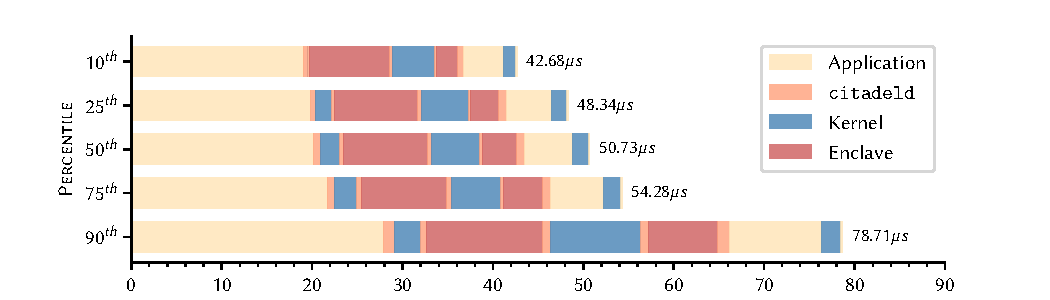
\includegraphics[width=\linewidth]{figures/graphs/open-anatomy.pdf}
    \vspace{-5mm}
    \caption{Control flow inhabitation for \texttt{libcitadel}'s \texttt{c\_open()} function, $n=100$.}
    \label{fig:open-anatomy}
\end{figure}


\begin{table}
    \centering
    \newcommand\tableTop{\rule{0pt}{3ex}}
    \newcommand\tableMid{\rule{0pt}{3ex}}
    \newcommand\tableBottom{\rule[-2ex]{0pt}{0pt}}
    \newcolumntype{N}{>{\centering\arraybackslash}m{2.5in}}
    
    \renewcommand\theadfont{\normalsize}
    \renewcommand\arraystretch{1.3}
    \begin{tabular}{l@{\hskip 0.15in} r@{\hskip 0.6in} r@{\hskip 0.35in} r@{\hskip 0.35in} r} 
        
        \toprule
        & \thead{\multirow{2}{*}{\textsc{Native}}} & \multicolumn{3}{c}{\thead{\textsc{Citadel}}} \\
        \cline{3-5}
        &  & \thead{\textit{Amortised}} & \thead{\textit{Cache Miss}} & \thead{\textit{$99^{th}$ \%ile}} \\
        % \cline{1-4}
        \midrule 
        \texttt{open()} & $1.675\pm0.076$ & $6.083\pm0.129$ & $50.133\pm1.482$ & $2.38\times$\\
        \texttt{read()} & $5.724\pm0.206$ & $7.010\pm0.192$ & $54.736\pm1.556$ & $1.26\times$\\
        \texttt{write()} & $14.340\pm0.208$ & $15.597\pm0.250$ & $63.824\pm1.902$ & $1.05\times$\\
        \texttt{close()} & $0.651\pm0.005$ & \multicolumn{2}{c}{$0.718\pm0.011$} & $1.10\times$\\

        

        \midrule 
        \texttt{socket()} & $1.446\pm0.179$ & \multicolumn{2}{c}{$3.156\pm0.291$} & $1.02\times$\\
        \texttt{bind()} & $0.762\pm0.023$ & $1.911\pm0.183$ & $49.110\pm1.746$ & $2.78\times$\\
        \texttt{listen()} & $0.705\pm0.015$ & $1.882\pm0.149$ & $48.411\pm1.386$ & $2.91\times$\\
        \texttt{connect()} & $16.570\pm0.278$ & $17.961\pm0.330$ & $66.273\pm2.147$ &$1.05\times$\\

        \midrule 
        \texttt{shmget()} & $1.880\pm0.122$ & $1.913\pm0.111$ & $49.326\pm1.466$ & $0.98\times$\\
        \texttt{shmat()} & $0.420\pm0.005$ & $1.575\pm0.134$ & $47.997\pm1.560$ & $0.99\times$\\
        \texttt{shmctl()} & $0.418\pm0.005$ & $0.743\pm0.083$ & $45.912\pm1.114$ & $0.97\times$\\
        \texttt{shmdt()} & $0.415\pm0.003$ & \multicolumn{2}{c}{$1.342\pm0.040$} & $1.01\times$\\



        \midrule 
        \texttt{pipe()} & $1.110\pm0.061$ & $1.288\pm0.069$ & $47.334\pm1.147$ & $1.02\times$\\
        \texttt{mkfifo()} & $3.865\pm0.048$ & $11.509\pm0.405$ & $59.623\pm1.788$ & $1.93\times$\\

        \midrule 
        \texttt{fork()} & $47.866\pm3.175$ & $48.647\pm3.457$ & $81.174\pm3.829$ & $15.77\times$\\
        \texttt{citadel\_init()} & $-$ & $0.801\pm0.009$ & $34.940\pm1.329$ & ---\\
        \bottomrule
    \end{tabular}
    \vspace{5mm}
    \captionsetup{justification=centering}
    \caption[\texttt{libcitadel} microbenchmarks]{\texttt{libcitadel} microbenchmarks. \\ All values are in $\mu s$ and the sample standard deviation is shown alongside the mean. For \textsc{Citadel}, both the amortised and average cache-miss durations are given. Only one value is given if the operation is not affected by a cache miss. The overhead between \textsc{Citadel} and Native Linux at the $99^{th}$ percentile is also presented. $n=10^6$.}
    \label{table:syscall-microbenchmarks}
\end{table}

\begin{figure}[h]
    \centering
    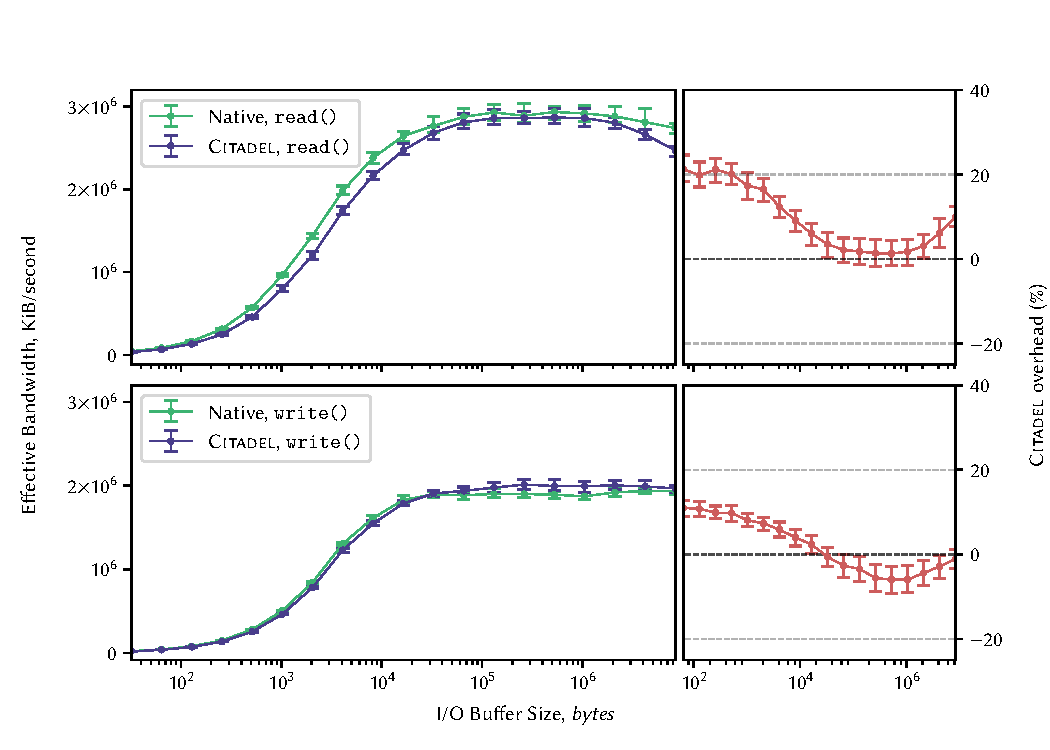
\includegraphics[width=\linewidth]{figures/graphs/io.pdf}
    \vspace{-5mm}
    \captionsetup{justification=centering}
    \caption[Effective \texttt{read()/write()} bandwidths for both the native Linux kernel and \textsc{Citadel}.]{Effective \texttt{read()/write()} bandwidths for both the native Linux kernel and \textsc{Citadel}. The percentage overhead is also presented. $n=200$ per buffer size.}
    \label{fig:io-graph}
\end{figure}

\paragraph{} A custom benchmark tool was built to assess the overall impact \textsc{Citadel} has on \textit{syscall} performance --- for example, the duration of \texttt{open()} compared to \texttt{c\_open()}. Table~\ref{table:syscall-microbenchmarks} presents these results. To give a fair comparison, two figures are reported for \textsc{Citadel}. \textit{Amortised} refers to the normal operation of \texttt{libcitadel}, in which the majority of queries are served from the cache; overhead arises from both local cache operations and added kernel latency from the \acrshort{lsm}. The other column, \textit{Cache Miss}, gives the overhead when caching is disabled, thus including communication with \texttt{citadeld}.

\paragraph{} Overall \texttt{libcitadel} contributes $\sim{}1 \mu s$ of overhead (amortised) on average --- this rises to $\sim$~$40 \mu s$ on a cache miss. Figure~\ref{fig:open-anatomy} presents a more detailed view of where exactly this overhead arises, approximately plotting where the control flow for \texttt{c\_open()} moves (on a cache miss). Interestingly, the slowest component is the communication channel between \texttt{libcitadel} and \texttt{citadeld} (median $26\mu s$);\footnote{Included in the \textit{Application} regions.} as a result, the core reference monitor functionality only adds a median penalty of $24\mu s$. The final \textit{Kernel} call before terminating is the internal call to \texttt{open()}. Additionally, the $10^{th}$ percentile demonstrates that the first \textit{Kernel} call is not always required if the entity's metadata is resident in the \texttt{citadeld} cache. During these experiments, \texttt{citadeld} showed to reliably handle over 30,000 requests/second and between $90-100\%$ usage of a single thread.

\paragraph{} Figure~\ref{fig:io-graph} plots observed effective bandwidth whilst reading from and writing to a 16 MiB file with different sized buffers; the corresponding percentage overhead inflicted by \textsc{Citadel} is plotted to the right. The benchmark driving this was adapted for Linux from one written by R.~Watson for FreeBSD.~\cite{l41-benchmark} The results clearly show \textsc{Citadel} having a more adverse effect on performance for smaller buffer sizes; unsurprising, as smaller buffers force a larger number of calls to \texttt{read()} / \texttt{write()}. It is unclear why \textsc{Citadel} provides better performance for large buffers with \texttt{write()}, an unexpected artefact --- the difference is statistically significant for buffers in the range $256$KiB and $2$ MiB, and reproducible. More work is required to determine the root causes, but hypotheses include the slight optimisation afforded by regular, small delays easing pressure on microarchitectural caches.





\subsection{IPC Microbenchmarks}
\label{sec:ipc-microbenchmarks}

\paragraph{} Again using the modified Watson benchmark, we investigated \textsc{Citadel}'s effect on end-to-end \acrshort{ipc} performance. We investigate \textit{pipes}, \textit{local sockets} (\texttt{socketpair()}), and \textit{regular sockets}, between 2 threads (Figure~\ref{fig:ipc-2thread-graph}) and between a parent and child process (Figure~\ref{fig:ipc-2proc-graph}).

\paragraph{} Overall, the results between the two contexts are similar --- both see approximately 20\% degradation in the worst cases, tending towards equal performance when using $\sim 10^5$-byte blocks. At first glance it appears that \textsc{Citadel} affects the performance between 2 threads slightly more than 2 processes, but in fact \textsc{Citadel} performs near-identically in both. Native performance is more heavily optimised when sending between two threads; \textsc{Citadel} overshadows any latency gained by the kernel.

\paragraph{} In a similar way to \texttt{write()}, \textsc{Citadel} unexpectedly outperforms the native kernel in both contexts using \texttt{pipe()}. The readings are noisy, but statistically significant for buffers in the range 16 KiB to 8 MiB, and reproducible. The cause is again unknown, but observing that the native kernel's throughput halves after buffers of 8 KiB, we suspect that this is the result of cache exhaustion or inopportune paging. Notably, \textsc{Citadel}'s readings exhibit a far larger \acrshort{iqr} for large buffer sizes than the native kernel, a side effect that is repeated in real-world testing.

\begin{figure}[]
    \centering
    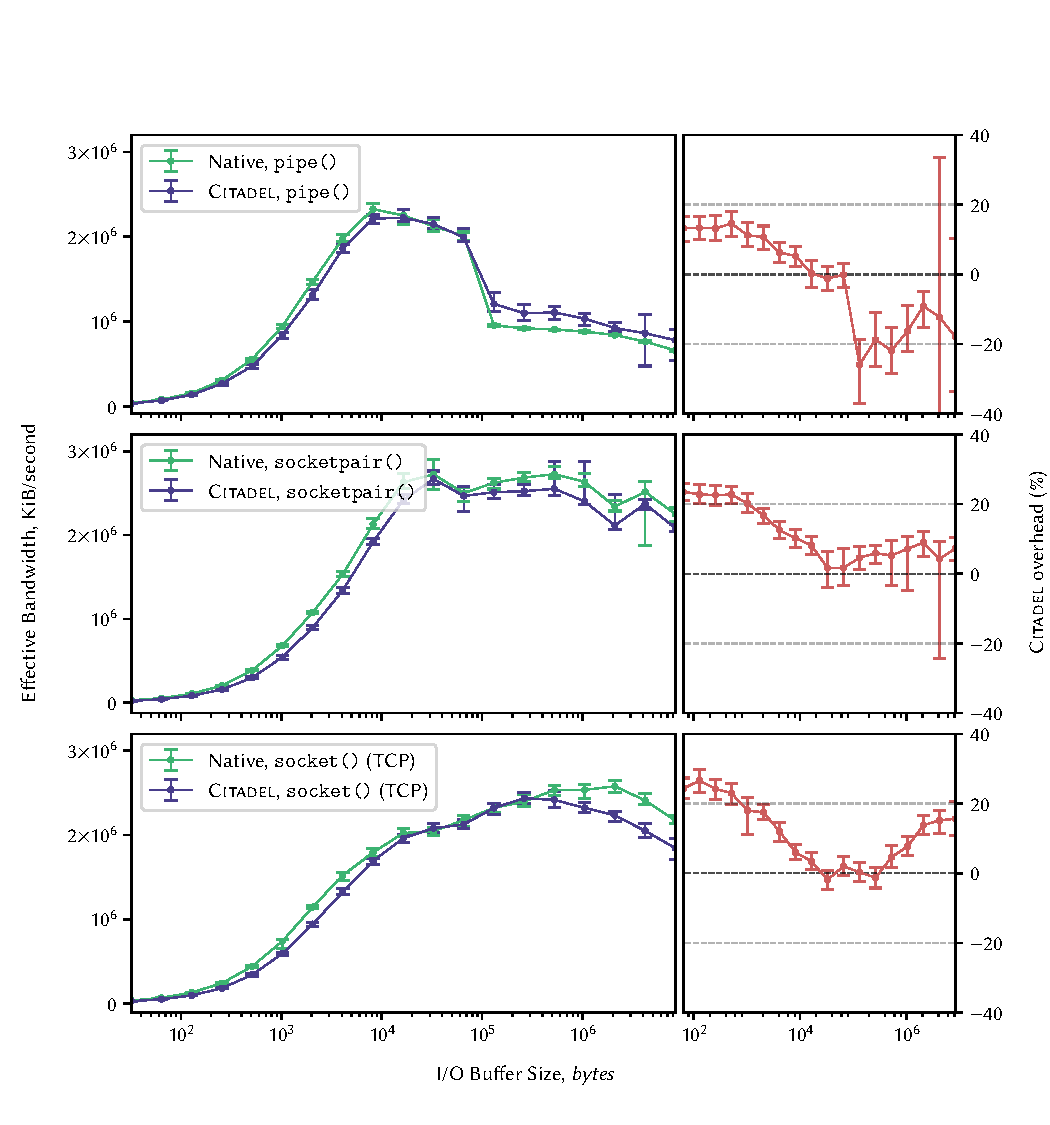
\includegraphics[width=\linewidth]{figures/graphs/ipc-2thread.pdf}
    \vspace{-5mm}
    \caption[Effective bandwidths for various types of IPC between \textit{2 threads}.]{Effective bandwidths for various types of \acrshort{ipc} between \textit{2 threads}, $n=200$.}
    \label{fig:ipc-2thread-graph}
\end{figure}


\begin{figure}[]
    \centering
    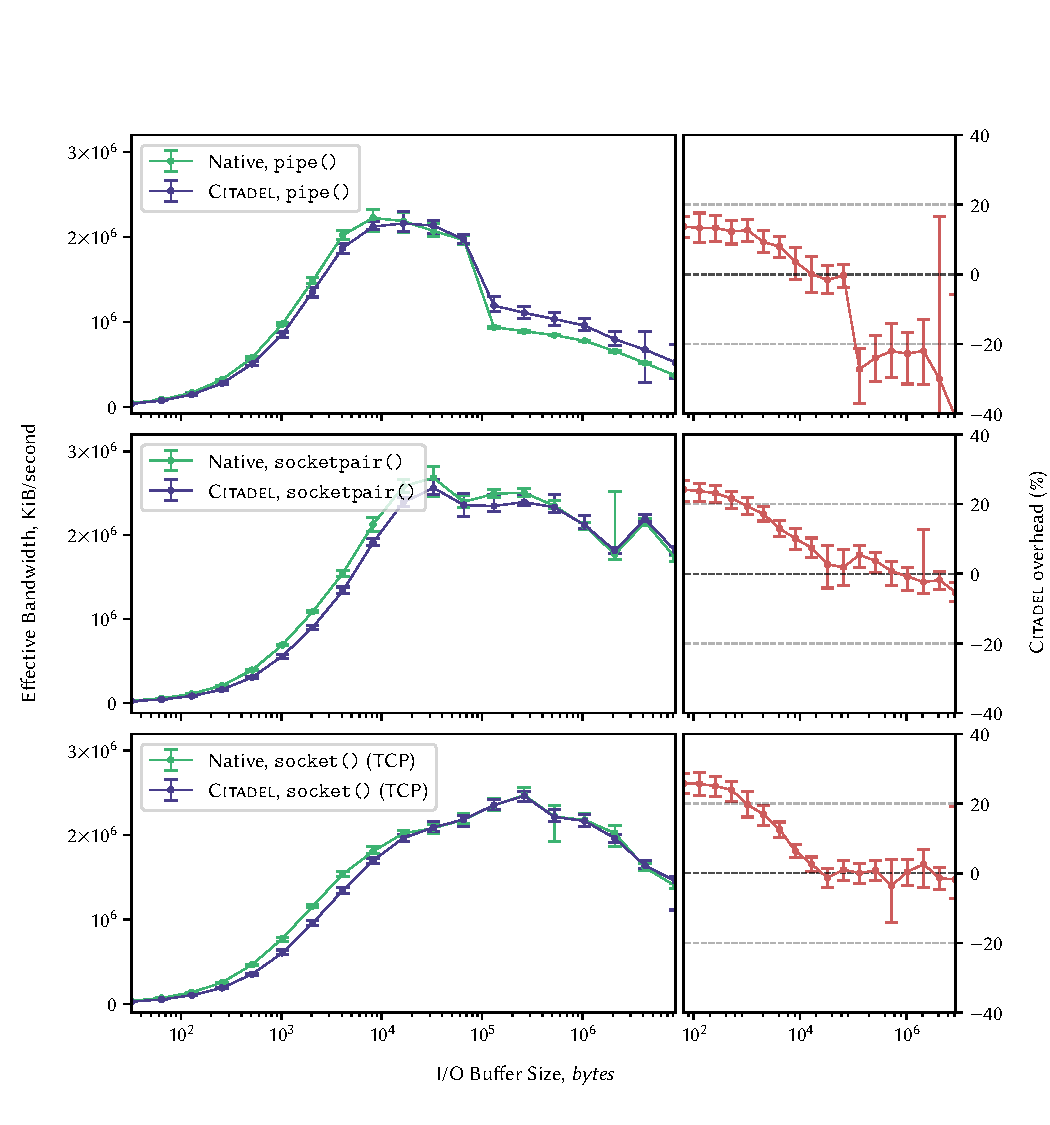
\includegraphics[width=\linewidth]{figures/graphs/ipc-2proc.pdf}
    \vspace{-5mm}
    \caption[Effective bandwidths for various types of IPC between \textit{2 processes}.]{Effective bandwidths for various types of \acrshort{ipc} between \textit{2 processes}, $n=200$.}
    \label{fig:ipc-2proc-graph}
\end{figure}

\clearpage

\subsection{\textsc{Nginx} Benchmarks}
\label{sec:nginx-benchmarks}
\begin{table}
    \centering
    \newcommand\tableTop{\rule{0pt}{3ex}}
    \newcommand\tableMid{\rule{0pt}{3ex}}
    \newcommand\tableBottom{\rule[-2ex]{0pt}{0pt}}
    \newcolumntype{N}{>{\centering\arraybackslash}m{2.5in}}
    
    \renewcommand\theadfont{\normalsize}
    \renewcommand\arraystretch{1.3}
    \begin{tabular}{l@{\hskip 0.35in} r@{\hskip 0.3in} r@{\hskip 0.35in} r@{\hskip 0.35in} c} 
        
        \toprule
        & \thead{\multirow{2}{*}{\textsc{Native}}} & \multicolumn{3}{c}{\thead{\textsc{Citadel}}} \\
        \cline{3-5}
        &  & \thead{\textit{Untainted}} & \thead{\textit{Tainted}} & \thead{\textit{Overhead}} \\
        % \cline{1-4}
        \midrule 
        \multicolumn{5}{l}{\textsc{Webserver Benchmark}, \textit{100-byte packets}} \\
        \textit{Latency} & $35.73\mu s$ & $36.18\mu s$ & $44.35\mu s$ & $24\%$ \\
        $-\;$ \textit{std. dev.} & $13.85\mu s$ & $14.12\mu s$ & $13.26\mu s$ & \\
        $-\;$ \textit{max.} & $536\mu s$ & $554\mu s$ & $508\mu s$ & \\
        \textit{Requests/s} & $2.748 \cdot 10^4$ & $2.717 \cdot 10^4$ & $2.214 \cdot 10^4$ & $19\%$\\
        \textit{Bandwidth} & $177.28$ Mbps & $168.72$ Mbps & $143.04$ Mbps & $18\%$\\

        \midrule 
        \multicolumn{5}{l}{\textsc{10GB File Transfer}} \\
        \textit{Bandwidth} & $1.404$ Gbps & $1.410$ Gbps & $1.413$ Gbps & $\sim 0\%$ \\
        $-\;$ \textit{std. dev.} & $0.428$ Gbps & $0.440$ Gbps & $0.549$ Gbps &\\
        \textit{Duration} & $56.98 s$ & $56.74 s$ & $56.62 s$ & $\sim 0\%$ \\
        $-\;$ \textit{std. dev.} & $19.45 s$ & $18.97 s$ & $23.63 s$ & \\
        
        \bottomrule
    \end{tabular}

    \vspace{5mm}
    \captionsetup{justification=centering}
    \caption[\textsc{Nginx} performance comparinson between native Linux, and both untainted and tainted \textsc{Citadel}.]{\textsc{Nginx} performance comparinson between native Linux, and both untainted and tainted \textsc{Citadel}, $n=25$.}
    \label{table:nginx-benchmarks}
\end{table}

\paragraph{} To validate the performance results presented thusfar, we ported the entirety of the \textsc{Nginx} webserver\footnote{\url{https://www.nginx.com/}} to function alongside \textsc{Citadel}. No optimisations were made to the codebase --- the only changes made replaced core \texttt{libc} function calls to use their \texttt{c\_*} \texttt{libcitadel} counterparts.

\paragraph{} Two trials were run; a low-latency benchmark\footnote{\url{https://github.com/wg/wrk}} and a 10GB \acrshort{http} file transfer (high-bandwidth). The webserver was configured to only run a single server process to ensure it was exercised to its full extent, and was set up to use the \textit{loopback} interface\footnote{\texttt{http://127.0.0.1/}.} to eliminate any interference from outside the \acrshort{os}. 

\paragraph{} The results are not surprising (Table~\ref{table:nginx-benchmarks}). For the low latency tests we observe the same $20-25$\% overhead as seen from \acrshort{tcp} sockets in §~\ref{sec:ipc-microbenchmarks} using the same buffer size. The high-bandwidth tests show \textsc{Citadel} performing equally to the native kernel, only differing by its larger sample standard deviation. This trial is also interesting as this is the first time we see file descriptor revalidation happening automatically on \texttt{read()} and \texttt{write()}. The \acrshort{cpu} overhead from \texttt{citadeld} was $<1\%$.





\section{Security}

\subsection{\textsc{Citadel} TCB}
\label{sec:citadel-tcb}

\paragraph{} One of the core initial goals of this project was to build an enclave-based reference monitor whilst \textit{minimising inflation to the system's \acrshort{tcb}}; to this end we present the trusted components of a \textsc{Citadel} system.

\begin{itemize}
    \item[---] The \acrshort{sgx} Platform, including all libraries and \textit{isgx}. 
    \item[---] The \textit{policy enclave} implementation.
    \item[---] The untrusted \texttt{citadeld} application; discussed further below.
    \item[---] The core Linux kernel, including the \textsc{Citadel} \acrshort{lsm} and the Linux \acrshort{vfs}.   
    \item[---] The Intel \textit{\acrshort{aesni}} Linux driver. 
\end{itemize}

\paragraph{} We also assume that the build environment is entirely trusted. A notable exclusion from the \acrshort{tcb} is the majority of Linux drivers and other kernel modules --- this was a strong motivation for using \acrshort{sgx}, as it can effectively defend against malicious and misbehaving ring-0 parties. 

\paragraph{} However, how might the system defend against \texttt{citadeld}, an un\-privileged, user\-space application, being replaced by a malicious adversary?

% \begin{enumerate}
%     \item How does the system defend against \texttt{citadeld}, an unprivileged, userspace application, from being replaced by a malicious adversary?
%     \item Can the kernel actually be held to the same integrity level as an enclave? Additionally, by extension, how trustable is a system that enclaves can only attest to half of?
% \end{enumerate}

\paragraph{} The compiled \texttt{citadeld} application could be protected in exactly the same way that \textsc{Citadel} defends its socket, \texttt{/run/citadel.socket}, with a reserved identifier. For example, opting to mark it with an \textit{\acrshort{xattr}} such as \texttt{security.citadel.daemon} with a \textit{nonce} value during the build process provides the \acrshort{lsm} ample confidence that an executable is a valid product of a \textsc{Citadel} build,\footnote{Using the \texttt{bprm\_check\_security} \acrshort{lsm} hook.} and protects it from tampering. This may also be valuable for defending the enclave object files themselves; although they cannot be tampered with, an adversary may try to remove them to deny service. These features would require extending the \textsc{Citadel} build system further.

\paragraph{} Secondly, can the kernel actually be held to the same integrity level as an enclave? How trustable is a system that enclaves can only attest to half of?

\paragraph{} Enclaves are unique in that their online attestation process inspires absolute trust, but offline provenance can be equally valuable. Although not \acrshort{sgx}-based, \textit{\acrshort{uefi} Secure Boot}~\cite{Richardson2013UefiSB} is an industry-standard mechanism for verifying whether an \acrshort{os} is legitimate. Ensuring that a \textsc{Citadel} system's installation is properly signed by a trusted party defends against many types of attack. 

\paragraph{} One example that \textsc{Citadel} cannot defend against has a malicious superuser compiling a new kernel with a modified \acrshort{lsm}, using valid keys scraped from the Linux system binary, and booting into it to bypass \textsc{Citadel}'s protections. Although not a bespoke solution, verifying an \acrshort{os} is well-explored and thus not a direct concern for this work. Additional protections include Linux's \textit{\acrlong{ima}} (§~\ref{sec:ima}).

\paragraph{} Thirdly, does the kernel protects itself adequately from malicious kernel modules?

\paragraph{} Effective protection is possible if carefully executed. Appendix~\ref{appendix:pid-tampering} presents a proof of concept kernel module that changes a process's \acrshort{pid} dynamically. This is highly concerning, as a process's \acrshort{pid} is its core identifier in \textsc{Citadel}'s eyes; defence was discussed in §~\ref{sec:pid-protection}. The Linux kernel is a soup of \textit{exported} and \textit{unexported symbols},\footnote{Symbols include functions and variables held in the global namespace; exporting is the process of exposing it publicly to be called by third parties.} which is exploitable to access internal functions never designed to be called from a different context. This work does not assess the implications for the \acrshort{lsm} framework, but highlights the potential need for \textit{defensive programming} when designing the \acrshort{lsm}.

\paragraph{} We believe that \textsc{Citadel}, with its restricted \acrshort{tcb}, can be trustworthy, creating a system of integrity checks based upon, and complementing, the trust placed in \acrshort{sgx} itself.

\subsection{IFC Model Implications}
\label{sec:ifc-model-implications}

\paragraph{} The \textsc{Citadel} \acrshort{ifc} model deviates from the designs and implementations of Pasquier et al. and Krohn et al. in three key ways;
\begin{enumerate}
    \item Policy and enforcement decision are separated.
    \item Passive entities may exist in a temporary \textit{transient} state.
    \item Operations between untainted entities are not mediated.
\end{enumerate}

\paragraph{} The first is handled with an extension to the core model to make policy decisions explicit and communicable (§~\ref{sec:permissible-operations}). This relationship is the core focus of this work, and \textsc{Citadel} at all points relies on conservative assumptions --- if not explicitly granted, permission is withheld. By default the system tends towards complete lockdown, a defensive measure to preserve \textit{safety} if subjected to denial of service.

\paragraph{} The second point is justified with an extension to the \textit{creation flow} rule (§~\ref{sec:permissible-operations}, (\ref{eqn:new-creation})). Transient entities are only created from a secure context, under which it automatically assumes the labelling of its parent entity. This may informally be considered an extension of the process's internal state, and held to the same restrictions. Such entities may only alter their security context (via another active entity) after being declared explicitly, leaving their transient states. 

\paragraph{} Regarding the final point --- tainting in \textsc{Citadel} assumes the worst, treating any potential infraction as cause for mediation; only the policy enclave may clear a taint. Assuming that all sensitive entities are correctly labelled, \textsc{Citadel} will protect them against anything within the system. Unlabelled entities are assumed to be in the public domain, which allows normal execution and access control to proceed until the taint boundary is crossed.

\subsection{SGX Vulnerabilities}
\label{sec:sgx-vulnerabilities}
\paragraph{} This work assume that the \acrshort{sgx} platform is itself secure; a successful attack on \acrshort{sgx} obviously compromises any protection offered by \textsc{Citadel}. A number of \acrshort{sgx} vulnerabilities have been detailed;~\cite{lipp2018meltdown, vanbulck2018foreshadow, Schwarz2019ZombieLoad, ridl, vanbulck2020lvi} these are effective and highly concerning, but mitigating them is not in the scope of this project.

\section{Use Cases}

\paragraph{} In the introduction, we laid out the motivation and goals for \textsc{Citadel}, including using it as a platform for reasoning about the relationship between an enclave and its host. Standard workflows for creating an \acrshort{sgx} application uses a library \acrshort{os}, such as \textit{SGX-LKL}~\cite{priebe2019sgxlkl} and \textit{Graphene-SGX},~\cite{203255} to create a synthetic Linux environment inside the enclave supporting the primary application --- this approach subjects the enclave to some of the same flaws and issues as the underlying \acrshort{os}. Could we reach a point where the host \acrshort{os} is trusted to hold custody of sensitive assets, instead of a trend toward pure isolation?

\paragraph{} Two hypothetical scenarios are presented --- one requiring secrecy, and one integrity --- to illustrate how \textsc{Citadel} could aid enclave-application development.

\paragraph{Scenario 1} A social-media company provides a \acrshort{gdpr} platform, through which members request an archive of their data and other assets; these may be over 10~GB. Processing and collation happen inside an enclave, and an external service authenticates requests. Must the enclave seal archives after creation, before storage, and unseal them when requested? A solution using \textsc{Citadel} may offload unencrypted archives to the custody of the host \acrshort{os}, using \acrshort{ifc}'s secrecy mechanic to prevent unauthorised release. On request, the webserver requests permission to declassify the archive from the authentication authority --- no penalty need be paid for encryption.\footnote{Disk encryption should be used for offline protection.}


\paragraph{Scenario 2} An Apache Spark application partitions input data into a large number of shards. Assuming that shard-processing is protected inside an enclave, do shards need to be cryptographically signed to verify their provenance? \textsc{Citadel} would entrust this tracking to the policy enclave, which, once attested, may be considered a part of the application's trusted components.

\paragraph{} Although \textsc{Citadel} may not be suitable for the most sensitive processing tasks --- enclaves are still vital here --- it offers a lightweight protection mechanism that could potentially be, in the interest of performance, trusted in a supporting role.
